%\chapter{Architektur}
\chapter{\colorbox{yellow}{Architektur}}

\section{Konzept}
%\section{\colorbox{green}{Konzept}}

\begin{wrapfigure}{l}{0.4\textwidth}
\begin{center}
\vspace{-40pt}%
 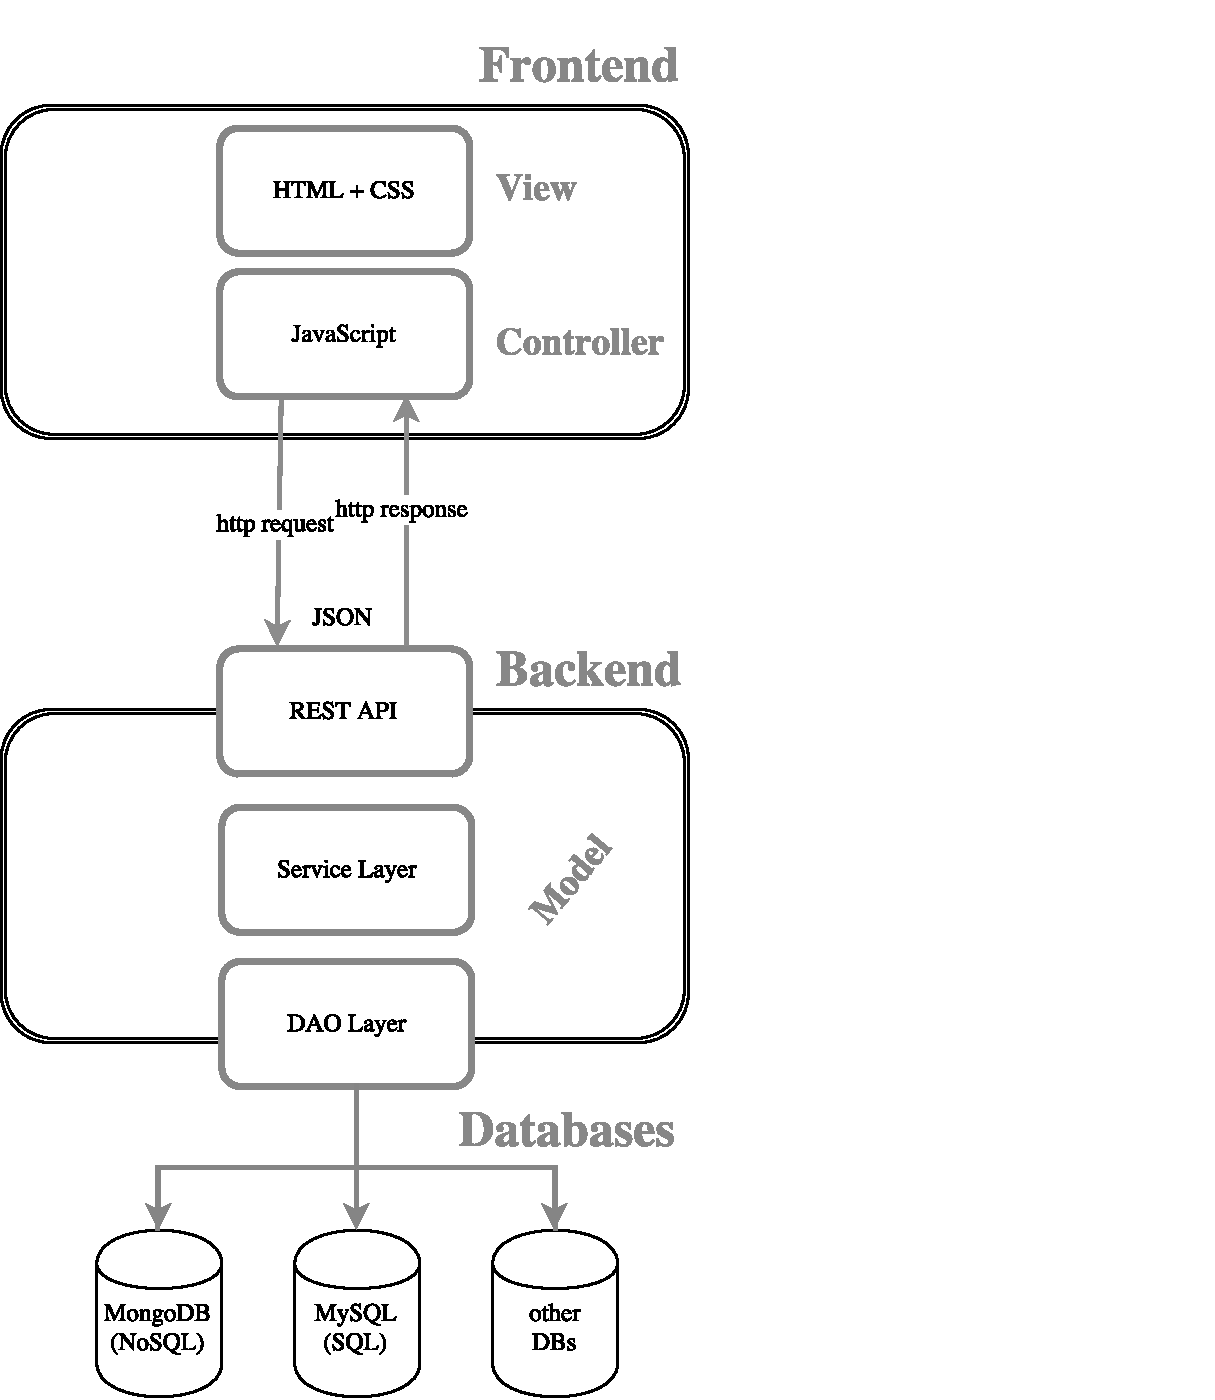
\includegraphics[trim = 0mm 0mm 0mm 0mm, clip, width=0.4\textwidth]{resources/architectureMyAppWithoutFrameworks}	
 \caption[Architektur-Prototyp]{Architektur-Prototyp}
 \label{img:architectureMyApp}
 \vspace{-70pt}%
 \end{center}
 \end{wrapfigure}


%
%
%\begin{figure}[H]
%%\vspace{-20pt}%
%\centering
%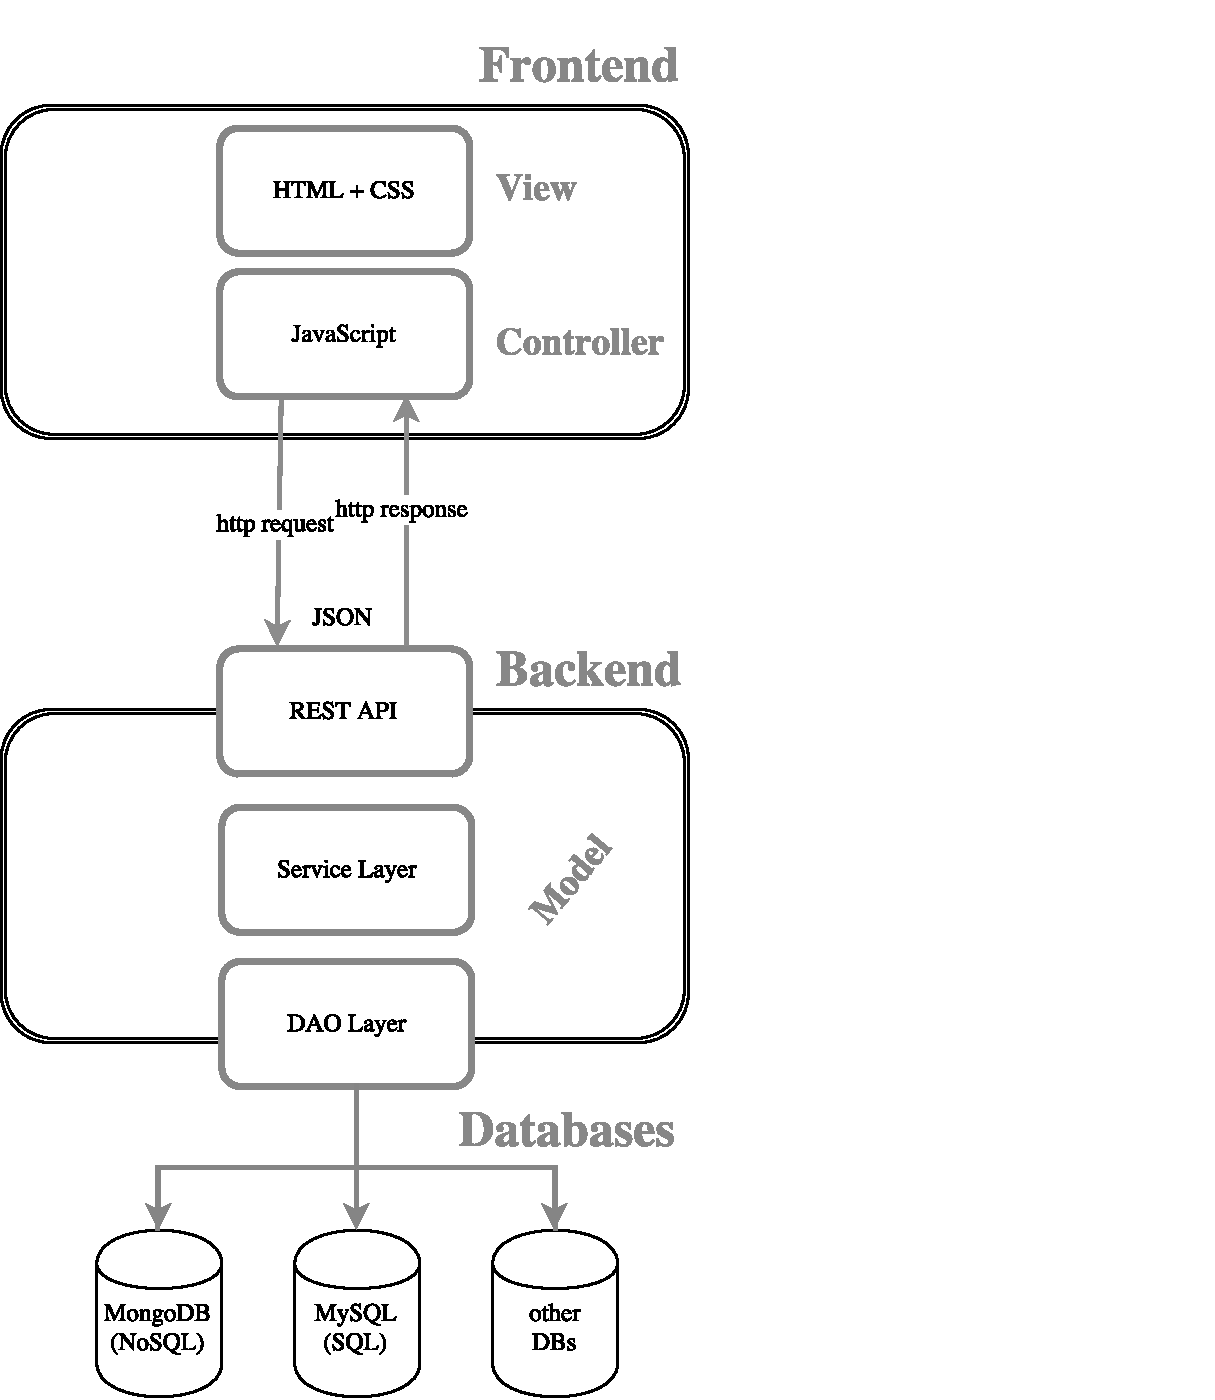
\includegraphics[trim = 0mm 0mm 0mm 0mm, clip, width=0.35\textwidth]{resources/architectureMyAppWithoutFrameworks}
%\caption[Architektur-Prototyp]{Architektur-Prototyp}
%\label{img:architectureMyApp}
%\end{figure}
Die vorgeschlagene Architektur ist auf der Abbildung \ref{img:architectureMyApp} zu sehen. Die Auswahl dieser Architektur hat zum Ziel, ein möglichst gutes Skalierungsverhalten der Anwendung zu erreichen. Die für die Performance zwei kritischen Komponenten - Backend-Server und die Datenbank - werden auf mehreren Rechnern verteilt. Der entscheidende Faktor für das Skalierungsverhalten beider Komponenten ist, wann und wie viel Synchronisation notwendig ist. 

In dieser Architektur wird das Ziel verfolgt, bei steigender Anzahl der Internetnutzer, sowohl für die Anfragen, die Leseoperationen in der Datenbank benötigen, als auch für die Anfragen, bei denen die Daten gespeichert werden müssen, die Antwortzeit konstant bleibt.

\subsection{Backend}
%\subsection{\colorbox{green}{Backend}}

Der Backend stellt seine Funktionalität als die Menge von Webservices mit \textit{REST}-Interface zu Verfügung.

\begin{figure}[H]
%\vspace{-20pt}%
\centering
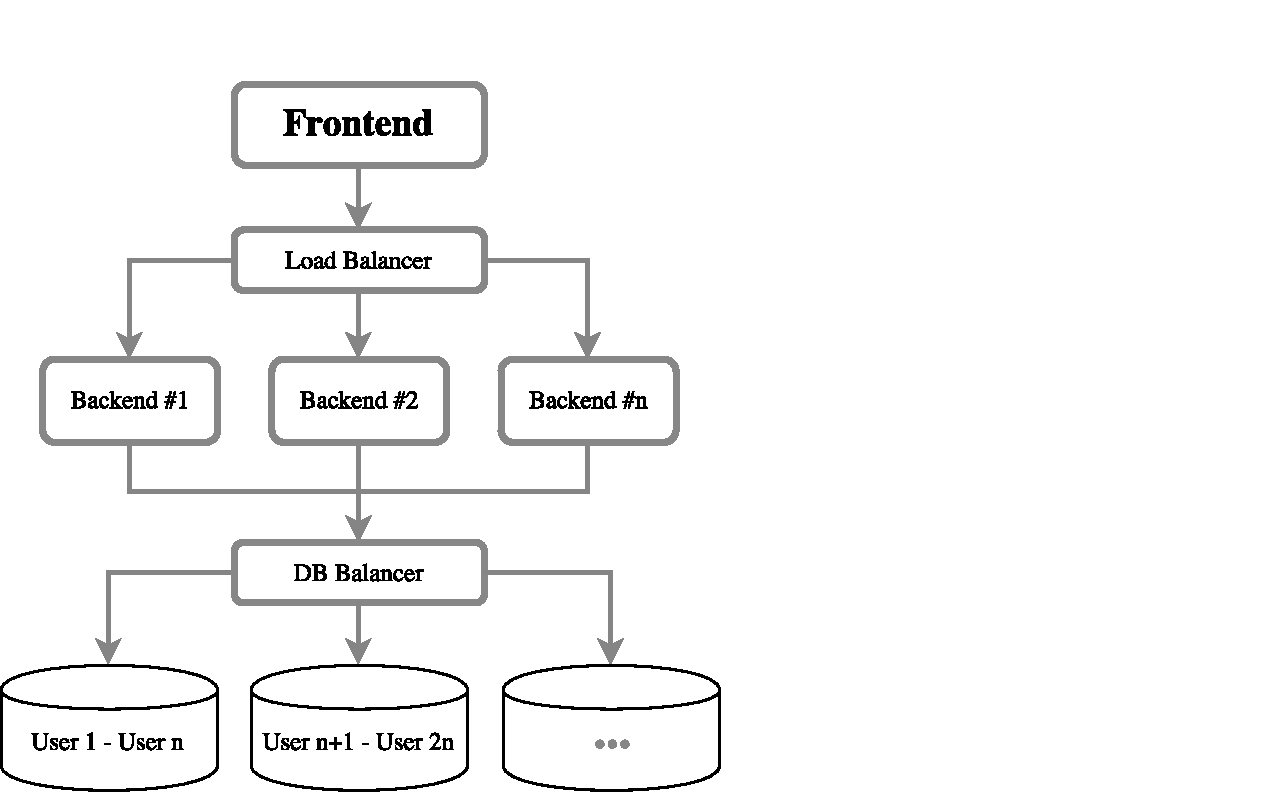
\includegraphics[trim = 0mm 0mm 0mm 0mm, clip, width=0.5\textwidth]{resources/ueberblickArchitektur}
\caption[Überblick zur vorgeschlagenen Architektur]{Überblick zur vorgeschlagenen Architektur}
\label{img:ueberblickArchitektur}
\end{figure}

Um ein gutes Skalierungsverhalten zu erreichen, wird jede Anfrage unabhängig von den anderen Anfragen bearbeitet. In dem Backend werden keine Informationen zwischengespeichert, alles was gespeichert werden muss, wird in die Datenbank geschrieben. Solche Komponente nennt man \textit{stateless}, weil sie keinen Zustand speichert. Somit ist keine Synchronisation zwischen den Maschinen des Backends notwendig, sogar die Anfragen innerhalb einer User-Session können von verschiedenen Maschinen bearbeitet werden. Ein \textit{Load Balancer} kann die Anfragen auf verschieden Maschinen in Backend verteilen ohne Rücksicht darauf nehmen zu müssen, welcher Maschine die jeweilige Anfrage entstammt.

Die Webservices sind unabhängig voneinander und können auch auf verschiedenen Maschinen ausgeführt werden. Diese Architektur ist auch als \textit{Microservice} Architektur bekannt.

%\subsection{\colorbox{green}{Datenbank}}
\subsection{Datenbank}

Das Skalierungskonzept für die Datenbank basiert auf der Annahme, dass die Webanwendung auf \textit{Multi-User} Betrieb ausgelegt ist und jeder User seine Daten unabhängig von den anderen Usern verwaltet. Daher ist es möglich, die Daten so aufzuteilen, dass sich alle Daten eines bestimmten Users nur in einem Teil der Daten wiederfinden. Dann ist es möglich, jeden Teil der Daten getrennt von allen anderen Teilen, z. B. auf eigener Maschine, zu speichern. Wenn der Backend-Server eine Anfrage bearbeitet, sind die Daten nur eines Nutzers betroffen. Damit fragt der Backend-Teil nur die Komponente ab, die entsprechenden Teil der Daten verwaltet. Es ist notwendig, diese Komponente zu identifizieren. Jedoch ist es eine billige \textit{Mapping}-Abfrage, z. B. von dem UserID zu der IP-Adresse der Maschine, die die Daten verwaltet. Während des \textit{Live}-Betriebs ist auch keine Synchronisation erforderlich. Die Synchronisation ist nur dann relevant, wenn die Daten neu aufgeteilt werden müssen.

%\section{Umsetzung}
\section{\colorbox{yellow}{Umsetzung}}

Die Umsetzung einzelner Komponenten des Prototyps wird durch Einsatz verschiedener Programmiersprachen und Frameworks realisiert.

Für Web-Client wird das moderne Angular 2 - JavaScript Framework eingesetzt. Bei der Implementierung des Web-Servers kommt das Spring Framework zum Einsatz. Mit dem Spring Framework werden mehrere Konzepte umgesetzt, so wie \textit{REST API}, \textit{Dependency Injection Pattern} und die Möglichkeit den Backend-Teil des Prototyps als ein \textit{Self-Contained} System zu betrachten. Die Persistenz und die Skalierung der Daten wird durch die NoSQL-Datenbank \mongo\ realisiert.

Der Prototyp wird so konzipiert, dass möglicher Ersatz einzelner Komponenten ohne großen Aufwand ermöglicht wird.

%\subsection{Implementierung}
\section{\colorbox{red}{Implementierung}}

%\subsection{Datenbank}
\subsection{\colorbox{yellow}{Datenbank}}

Der Backend-Teil des Prototyps wird in Java implementiert. Um alle verfügbaren \mongo-Operationen in Java nutzen zu können, muss zuerst der entsprechende Treiber geholt werden.

Der Java \mongo-Treiber kann beispielsweise durch Maven-Konfigurationsdatei \texttt{pom.xml} als Abhängigkeit deklariert werden, um benötigte Bibliotheken automatisch herunterzuladen. In Fall des Prototyps wird der MongoDB Java Treiber benötigt.

\begin{listingsboxJava}[label={lst:pom}]{myxml}{MongoDB Java Treiber als Maven Dependency, Version 3.4.2}
	<!-- Mongo Java Driver -->
	<dependency>
		<groupId>org.mongodb</groupId>
		<artifactId>mongo-java-driver</artifactId>
		<version>3.4.2</version>
	</dependency>
\end{listingsboxJava}

Für die Kommunikation mit einer Datenbank und ihren \textit{Collections}, die auf einem einzigen Server abgelegt sind, reicht in Java-Klasse Folgendes zu deklarieren:
\begin{listingsboxJava}[label={lst:conn}]{myJava}{Verbindungsaufbau mit einem Server}
public static void main(String[] args) {

	MongoClient mongoClient = new MongoClient("localhost", 27017);
	MongoDatabase db = mongoClient.getDatabase("qwertz");
	MongoCollection<Document> collectionOfUsers = db.getCollection("users");
        
        // weitere CRUD-Operationen mit der ausgewählten Collection
}
\end{listingsboxJava}

Falls die Daten auf einem einzigen Server abgelegt werden, kann inzwischen beim Serverausfall vorkommen, dass die Daten für eine ungewisse Zeit gar nicht verfügbar sind. Um die Verfügbarkeit der Daten auch beim Serverausfall zu garantieren, wird in dem Prototyp eine Replikationsgruppe mit insgesamt  3-Servern erzeugt.

\subsubsection{\colorbox{yellow}{Replikation (Replication)}}
%\subsubsection{Replikation (Replication)}

Eine Replikatioinsgruppe anzulegen, ist es nur über die sog. \textit{Mongo Shell} auf der Kommandozeile möglich. Um die Replikationsgruppe effizienter erzeugen zu können, wird zuerst ein Skript \ref{lst:scriptForCreateOfRep} geschrieben. Das Skript legt neue Ordner an, welche unter Anderem die log-Dateien jeweiliger Server enthalten werden.

\begin{listingsboxShell}[label={lst:scriptForCreateOfRep}]{myshell}{Skript zum Erstellen einer Replikationsgruppe}
// create_replica_set.sh
#!/usr/bin/env bash

mkdir -p /data/rs1 /data/rs2 /data/rs3

// Start von drei lokalen mongod-Instanzen als Replikationsgruppe

mongod --replSet m101 --logpath "1.log" --dbpath /data/rs1 --port 27017
--oplogSize 64 --fork --smallfiles
mongod --replSet m101 --logpath "2.log" --dbpath /data/rs2 --port 27018
--oplogSize 64 --smallfiles --fork
mongod --replSet m101 --logpath "3.log" --dbpath /data/rs3 --port 27019
--oplogSize 64 --smallfiles --fork
\end{listingsboxShell}

Das Skript mit dem Inhalt aus Listing \ref{lst:scriptForCreateOfRep} wird folgendermaßen ausgeführt:

\begin{listingsboxShell}[label={lst:runOfscriptForCreateOfRep}]{myshell}{Erstellen einer Replikationsgruppe anhand eines Skriptes}
vlfa:scripts vlfa$ bash < create_replica_set.sh
\end{listingsboxShell}

%Damit ist die Konfigurationsgruppe mit 3 Servern angelegt. Zum Anschauen einer log-Datei;
%
%\begin{listingsboxShell}[label={lst:X}]{myshell}{1.log-Inhalt}
%2016-12-19T14:58:11.637+0100 I CONTROL  [initandlisten] MongoDB starting :
%pid=25626 port=27017 dbpath=/data/rs1 64-bit host=vlfa.fritz.box
%// irrelevant
%2016-12-19T14:58:11.639+0100 I CONTROL  [initandlisten] options:
%{ net: { port: 27017 }, processManagement: { fork: true }, replication:
%{ oplogSizeMB: 64, replSet: "m101" }, storage: { dbPath: "/data/rs1",
%mmapv1: {smallFiles: true}}, systemLog: {destination: "file", path: "1.log"}}
%// irrelevant
%\end{listingsboxShell}

Die Replikationsgruppe muss man zusätzlich initialisieren:

\begin{listingsboxJavaScript}[label={lst:initReplica}]{myJS}{Skript zur Initialisierung der Replikationsgruppe}
// init_replica.js
config = { _id: "m101", members:[
          { _id : 0, host : "localhost:27017"},
          { _id : 1, host : "localhost:27018"},
          { _id : 2, host : "localhost:27019"} ]
};

rs.initiate(config);
rs.status();
\end{listingsboxJavaScript}

\begin{listingsboxShell}[label={lst:runOfInitReplica}]{myshell}{Skript ausführen}
vlfa:scripts vlfa$ mongo --port 27018 < init_replica.js
\end{listingsboxShell}

Die Server aus Listing \ref{lst:initReplica} nehmen nun Kontakt miteinander auf, gründen die Gruppe und wählen den Primary-Server aus. Den Zustand der Replikationsgruppe ist es möglich, mit \texttt{rs.status()} zu überprüfen. Beim Ausfall des Primary-Servers wählen die Secondaries untereinander entsprechend einen neuen Primary-Server aus. Damit wird die Ausfallsicherheit des Servers erreicht. Die Mindestanzahl an Servern in einer Replikationsgruppe liegt bei drei. 

Nachdem die Replikationsgruppe angelegt ist, kann drauf zugegriffen werden. Listing \ref{lst:javaZugriff} veranschaulicht das Beispiel.

\begin{listingsboxJava}[label={lst:javaZugriff}]{myJava}{Initialisierung einer Replikationsgruppe}
public static void main (String[] args) throws InterruptedException {
        MongoClient client = new MongoClient(asList(
                new ServerAddress("localhost", 27017),
                new ServerAddress("localhost", 27018),
                new ServerAddress("localhost", 27019)));
                
                // weitere CRUD-Operationen
}
\end{listingsboxJava}

%\begin{listingsboxShell}[label={lst:X}]{myshell}{Simulation des Server-Ausfalls 'PRIMARY' über Shell}
%m101:PRIMARY> rs.stepDown()
%
%Result:
%
%2016-12-19T21:24:12.739+0100 I NETWORK  [thread1]
%trying reconnect to 127.0.0.1:27018 (127.0.0.1) failed
%2016-12-19T21:24:12.760+0100 I NETWORK  [thread1]
%reconnect 127.0.0.1:27018 (127.0.0.1) ok
%m101:SECONDARY> 
%\end{listingsboxShell}

Um die Sicherung der Zugehörigkeit der Mitglieder zu konkreter Replikationsgruppe festzustellen, kann der Code aus Listing \ref{lst:javaZugriff} entsprechend erweitert werden, Zeilen 6-8.
\begin{listingsboxJava}[label={lst:guarantee}]{myJava}{Sicherung der Zugehörigkeit zu konkreter Replikationsgruppe}
 public static void main (String[] args) throws InterruptedException {
        MongoClient client = new MongoClient(asList(
                new ServerAddress("localhost", 27017),
                new ServerAddress("localhost", 27018),
                new ServerAddress("localhost", 27019)), 
                MongoClientOptions.builder()
                        .requiredReplicaSetName("m101")
                        .build());
\end{listingsboxJava}

Um die Daten auf mehreren Servern zu verteilen, wird in dem Prototyp die horizontale Skalierung umgesetzt.

\subsubsection{\colorbox{red}{Skalierung (Sharding)}}
%\subsubsection{Skalierung (Sharding)}
blablabla

%\subsection{Web-Server}
\subsection{\colorbox{yellow}{Web-Server}}

%\begin{listingsboxJava}[label={lst:X}]{myJava}{}
%
%\end{listingsboxJava}
In der Spring-basierten Webanwendung muss der Spring Core Container, in dem Beans definiert sind und diese per Dependency Injection zusammengebracht werden, über einen \texttt{ApplicationContext} erzeugt werden.
\begin{listingsboxJava}[label={lst:X}]{myJava}{Webanwendung starten}
import org.springframework.boot.SpringApplication;
import org.springframework.boot.autoconfigure.SpringBootApplication;

@SpringBootApplication
public class Application {

    public static void main(String[] args) throws Exception {
        SpringApplication.run(Application.class, args);
    }
}
\end{listingsboxJava}
Die \texttt{@SpringBootApplication}-Annotation fasst insgesamt die drei Annotationen zusammen:
\begin{itemize}

\item \texttt{@Configuration} - deklariert eine Klasse als Konfigurationsklasse für Springs Java-basierende Konfiguration.
\item \texttt{@EnableAutoConfiguration} - aktiviert eine automatische Konfiguration durch Spring Boot.
\item \texttt{@ComponentScan} - scannt die weiteren per \texttt{@Controller-} oder \texttt{@Service}- annotierte Klassen, die über den \texttt{ApplicationContext} erzeugt werden.\footnote{Spring Boot, \url{http://www.torsten-horn.de/techdocs/Spring-Boot.html}, zugegriffen am 29. Januar 2017}

\end{itemize}

@Configuration: Definiert eine Klasse als Konfigurationsklasse für Springs Java-basierende Konfiguration (im Gegensatz zur XML-Konfiguration).
@EnableAutoConfiguration: Aktiviert die weitreichende automatische Konfiguration durch Spring Boot.
@ComponentScan: Aktiviert die Erkennung weiterer automatisch zu konfigurierender Klassen als Spring Beans im Spring Application Context, z.B. per @Controller annotierte Klassen.

%\subsection{Load Balancer}
\subsection{\colorbox{red}{Load Balancer}}

%\subsection{Web-Client}
\subsection{\colorbox{red}{Web-Client}}



